\documentclass[10pt]{article}
\usepackage[T1]{fontenc}
\usepackage{lmodern}
\usepackage[margin=0.7in]{geometry}
\usepackage{amsmath}
\usepackage{microtype}
\usepackage{graphicx}
\usepackage{float}
\usepackage{booktabs}
\usepackage[font=small,labelfont=bf,skip=3pt]{caption}
\captionsetup[figure]{font=footnotesize}
\usepackage[dvipsnames]{xcolor}
\usepackage[colorlinks=true,linkcolor=MidnightBlue,citecolor=MidnightBlue,urlcolor=MidnightBlue]{hyperref}
\usepackage[capitalise]{cleveref}
\setlength{\parskip}{2pt}
\setlength{\parindent}{0pt}
\setlength{\intextsep}{6pt}
\makeatletter
\renewcommand\paragraph{\@startsection{paragraph}{4}{\z@}{1.0ex \@plus .3ex \@minus .2ex}{-1em}{\normalfont\normalsize\bfseries}}
\renewcommand\maketitle{\begin{center}{\large\bfseries\@title\par}\vspace{3pt}\@author\quad\textperiodcentered\quad\@date\end{center}}
\makeatother

\title{Muon with a negative power of the singular values (MSE loss)}
\author{Juntang Wang and V\'ictor Conchello}
\date{November 15, 2026}

\begin{document}
\maketitle
\vspace{-0.8em}

\paragraph{Does a negative power $p$ help?} Yes, slightly. The final validation loss is lowest at $p=-0.3$ at both learning rates: 0.5628 against 0.5648 for standard Muon at rate 0.005. Rerun on two more data orders at that rate, it wins again (by 0.005 each). The loss rises on both sides of $p=-0.3$, steeply below $p=-0.5$ (\cref{tab:negp}). $p=-0.3$ is not faster at the start: it reaches training loss 0.65 at about the same step as standard Muon and gains afterwards (\cref{fig:negp}).

\paragraph{What $p$ is.} Muon writes its momentum matrix as $U\,\mathrm{diag}(s)\,V^\top$ (its SVD) and updates the weights by $U\,\mathrm{diag}(s^p)\,V^\top$, rescaled to the Frobenius norm of the $p=0$ update. $p=1$ is the momentum itself. $p=0$ gives every direction the same step: this is Muon with exact orthogonalization; standard Muon approximates it by a Newton--Schulz iteration (its own row in \cref{tab:negp}). $p<0$ gives the largest steps to the directions where the momentum is smallest.

\paragraph{Clamping rule ($p<0$ only).} Each singular value is divided by the largest one, and a ratio below $10^{-6}$ is replaced by $10^{-6}$ before the power is taken; $10^{-6}$ is about the accuracy of a single-precision SVD. Between steps 200 and 7000 the clamped directions carry 2 to 4\% of the squared norm of the update at $p=-0.3$, 7 to 13\% at $p=-0.5$ and 7 to 39\% at $p\le-0.75$. At $p\le-0.75$, from step 3000 on, each matrix's update is close to rank one: over half of it goes to one direction, clamped or not.

\paragraph{Runs.} A small GPT on TinyStories (the TinyStories-10M setup), MSE loss (squared error to the one-hot next token), 10{,}000 steps, data order 0 unless stated (the shuffling seed), learning rate 0.005 (the rate used for Muon with this loss) and half of it.

\begin{table}[H]
\centering
\small
\caption{Muon with singular values raised to $p$, data order 0. Stable rank ($\|W\|_F^2/\sigma_1^2$) and $\sigma_1/\sigma_{\mathrm{median}}$ are means over the 36 weight matrices, at the step where the training loss at rate 0.005 reaches 0.65 ($p=0.75$ ends at 0.652). A dash: not run.}
\label{tab:negp}
\begin{tabular}{l ccccc}
\toprule
    & step at training & stable & & final val.\ loss, & final val.\ loss, \\
run & loss 0.65 & rank & $\sigma_1/\sigma_{\mathrm{median}}$ & rate 0.005 & rate 0.0025 \\
\midrule
$p=-1$    & 3688 & 11.6 & 16.25 & 0.6052 & -- \\
$p=-0.75$ & 2930 & 15.5 & 11.07 & 0.5801 & -- \\
$p=-0.5$  & 2582 & 27.0 & 6.22 & 0.5635 & 0.5692 \\
$p=-0.3$  & 1966 & 68.3 & 3.05 & \textbf{0.5628} & \textbf{0.5630} \\
$p=-0.1$  & 2034 & 101.4 & 2.37 & 0.5671 & 0.5679 \\
$p=0$     & 2262 & 95.6 & 2.50 & 0.5710 & 0.5687 \\
$p=0.25$  & 3346 & 36.9 & 6.31 & 0.5928 & 0.5906 \\
$p=0.5$   & 7608 & 12.2 & 29.97 & 0.6366 & 0.6102 \\
$p=0.75$  & not reached & & & 0.6496 & 0.6270 \\
\midrule
Muon (Newton--Schulz) & 2032 & 84.8 & 2.89 & 0.5648 & 0.5691 \\
AdamW (rate 0.002) & 4637 & 18.5 & 14.86 & 0.5908 & -- \\
\bottomrule
\end{tabular}
\end{table}

\begin{figure}[H]
\centering
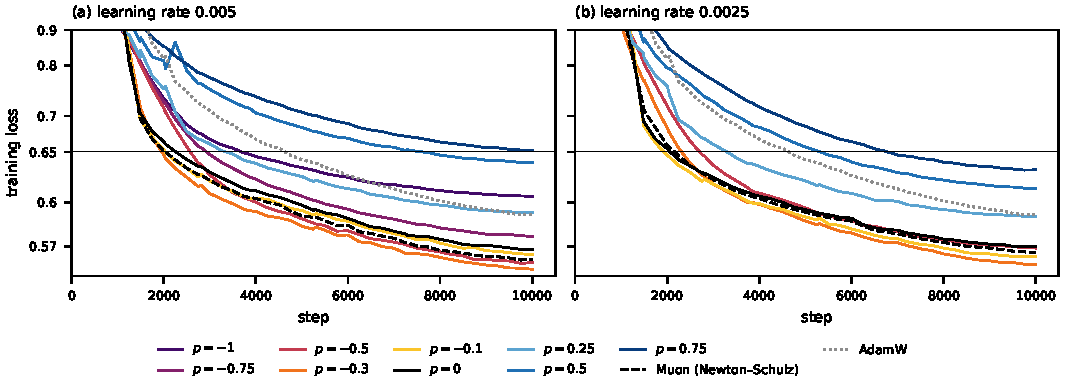
\includegraphics[width=\linewidth]{ts10m_mse/dose_loss.pdf}
\caption{Training loss, one colour per $p$ (yellow to dark purple: negative; blue: positive). The loss axis is logarithmic in (loss $-$ 0.5); the horizontal line is the loss 0.65 of \cref{tab:negp}. $p=-1$ and $p=-0.75$ were run at rate 0.005 only; AdamW has rate 0.002 in both panels.}
\label{fig:negp}
\end{figure}

\paragraph{Spectra.} The stable rank of the weights is highest at $p=-0.1$; the best run, $p=-0.3$, has a lower one than Muon (68 against 85).

\end{document}
